\documentclass{article}

\usepackage{siunitx} % Provides the \SI{}{} and \si{} command for typesetting SI units
\usepackage{graphicx} % Required for the inclusion of images
\usepackage{amsmath} % Required for some math elements 
\usepackage[export]{adjustbox} % loads also graphicx
\usepackage{listings}
\usepackage{matlab-prettifier}
\usepackage{float}
\usepackage[most]{tcolorbox}
\usepackage{amsfonts}
\usepackage{color}
\usepackage{titlesec}
\usepackage{caption}
\usepackage{subcaption}
\usepackage{placeins}

\newcommand{\R}{\mathbb{R}}

\usepackage{xcolor}

\DeclareCaptionFont{white}{\color{white}}
\DeclareCaptionFormat{listing}{%
  \parbox{\textwidth}{\colorbox{gray}{\parbox{\textwidth}{#1#2#3}}\vskip-4pt}}
\captionsetup[lstlisting]{format=listing,labelfont=white,textfont=white}
\lstset{frame=lrb,xleftmargin=\fboxsep,xrightmargin=-\fboxsep}
\titleformat{\section}[runin]
  {\normalfont\Large\bfseries}{\thesection}{1em}{}
\titleformat{\subsection}[runin]
  {\normalfont\large\bfseries}{\thesubsection}{1em}{}


\setlength\parindent{0pt} % Removes all indentation from paragraphs

\renewcommand{\labelenumi}{\alph{enumi}.} % Make numbering in the enumerate environment by letter rather than number (e.g. section 6)

%\usepackage{times} % Uncomment to use the Times New Roman font

%----------------------------------------------------------------------------------------
%	DOCUMENT INFORMATION
%----------------------------------------------------------------------------------------

\title{AMATH 353: Homework 14 \\Due May, 30 2018 \\ ID: 1064712} % Title

\author{Trent \textsc{Yarosevich}} % Author name

\date{\today} % Date for the report

\begin{document}
\maketitle % Insert the title, author and date
\setlength\parindent{1cm}

\begin{center}
\begin{tabular}{l r}
%Date Performed: December 1, 2017 \\ % Date the experiment was performed
Instructor: Jeremy Upsal % Instructor/supervisor
\end{tabular}
\end{center}

% If you wish to include an abstract, uncomment the lines below
% \begin{abstract}
% Abstract text
% \end{abstract}

%----------------------------------------------------------------------------------------
%	SECTION 1
%----------------------------------------------------------------------------------------
\section*{Part 1}
\subsection*{(a)}
Given the following initial condition, we get:
\begin{equation}
u(x,0)= 
  \begin{cases}
			\frac{\pi}{2}, \; \; \; x < 1 \\
			\frac{\pi}{4}, \; \; \; x \geq 1 \\
            \end{cases}
\
\end{equation}
\begin{equation}
\begin{aligned}
\frac{du}{dt} = 0\\
u(x(t), t) = A\\
A = u_0(x_0) = u(x, 0)\\
\end{aligned}
\end{equation}
We can then make use of $x(t) = x_0 + c(u_0(x_0)t$: and determine the equations for the characteristics:
\begin{equation}
\begin{aligned}
c(u(x(t), t)) = \sin(u)\\
c(u_0(x_0)) = \sin(u_0(x_0))\\
\end{aligned}
\end{equation}
\begin{equation}
c(u_0(x_0) 
  \begin{cases}
			1, \; \; \; x_0 < 1 \\
			\frac{\sqrt{2}}{2}, \; \; \; x_0 \geq 1 \\
            \end{cases}
\
\end{equation}
This in turn gives the following characteristics curves, and the solution along them:
\begin{tcolorbox}[minipage,colback=white,arc=0pt,outer arc=0pt]
\begin{equation}
x(t) = 
  \begin{cases}
			x_0 + t, \; \; \; x_0 < 1 \\
			x_0 + \frac{\sqrt{2}}{2}t, \; \; \; x_0 \geq 1 \\
            \end{cases}
\
u(x(t), t)= 
  \begin{cases}
			\frac{\pi}{2}, \; \; \; x_0 < 1 \\
			\frac{\pi}{4}, \; \; \; x_0 \geq 1 \\
            \end{cases}
\
\end{equation}
\end{tcolorbox}~
Additionally, here are the characteristics in different arrangements, which will be useful.
\begin{equation}
t = 
  \begin{cases}
			x - x_0, \; \; \; x_0 < 1 \\
			\sqrt{2}(x - x_0) \; \; \; x_0 \geq 1 \\
            \end{cases}
\
\end{equation}
\begin{equation}
x_0 =
  \begin{cases}
			x - t, \; \; \; x_0 < 1 \\
			x - \frac{\sqrt{2}}{2}t \; \; \; x_0 \geq 1 \\
            \end{cases}
\
\end{equation}
\subsection*{(b)}
%Also have to show that the slope to the left of the discontinuity are greater than those to the left.

Because $u(x(t), t) = u_0(x_0)$ we can find the breaking time by finding where its derivative goes to $\infty$. 
\begin{equation}
u_x = u_0'(x_0)\frac{dx_0}{dx}\\
\end{equation}
It is clear from the initial condition given above that $u_x$ blows up when we try to take the derivative $u_0'(x_0)$ because $u_0(x_0)$ has a discontinuity when $x_0 = 1$. Plugging this into equation (7) above at $t=0$ we see that this occurs at $x = 1$. Last, we need to confirm that when this discontinuity occurs, that the characteristic lines are actually crossing. Plugging in the value for $x_0$ we have:
\begin{equation}
t = 
  \begin{cases}
			x - 1, \; \; \; x_0 < 1 \\
			\sqrt{2}(x - 1) \; \; \; x_0 \geq 1 \\
            \end{cases}
\
\end{equation}
The slope of the characteristic line for $x_0 < 1$ is 1, and the slope for $x_0 \geq 1$ is $\sqrt(2)$. Both lines pass through $x = 1, t = 0$, so the lines will indeed cross at $t=0$. In the class we seem comfortable saying this, but technically, don't the characteristics cross at an infinitely small $t > 0$? In any case:
\begin{tcolorbox}[minipage,colback=white,arc=0pt,outer arc=0pt]
\begin{equation}
t_b = 0, \text{ at } x =1
\end{equation}
\end{tcolorbox}
\subsection*{(c)}
Since $\phi(x,t) = \sin(u)u_x$ we can integrate to get the following (note that I am ignoring the constant of integration, since it drops out in the Rankine-Hugoniot relation anyway):
\begin{equation}
\phi(x, t) = -\cos(u)
\end{equation}
We know from equation (2) above that $u^- = \frac{\pi}{2}$ and $u^+ = \frac{\pi}{4}$ giving:
\begin{equation}
\begin{aligned}
\frac{dx_s}{dt} = \frac{[\phi]}{[u]}\\
\frac{[\phi]}{[u]} = \frac{-\cos(u^+) + \cos(u^-)}{u^+ - u^-}\\
\frac{dx_s}{dt} = \frac{-\frac{\sqrt{2}}{2}}{-\frac{\pi}{4}}
\end{aligned}
\end{equation}
Which simplifies to:
\begin{equation}
\frac{dx_s}{dt} = \frac{2\sqrt{2}}{\pi}
\end{equation}
We then integrate and apply the initial condition found in (b):
\begin{tcolorbox}[minipage,colback=white,arc=0pt,outer arc=0pt]
\begin{equation}
\begin{aligned}
x_s(t) = \frac{2\sqrt{2}}{\pi}t + C\\
x_s(0) = 1 = C\\
x_s(t) = \frac{2\sqrt{2}}{\pi}t + 1
\end{aligned}
\end{equation}
\end{tcolorbox}
\begin{figure}[!htbp]
  \centering
    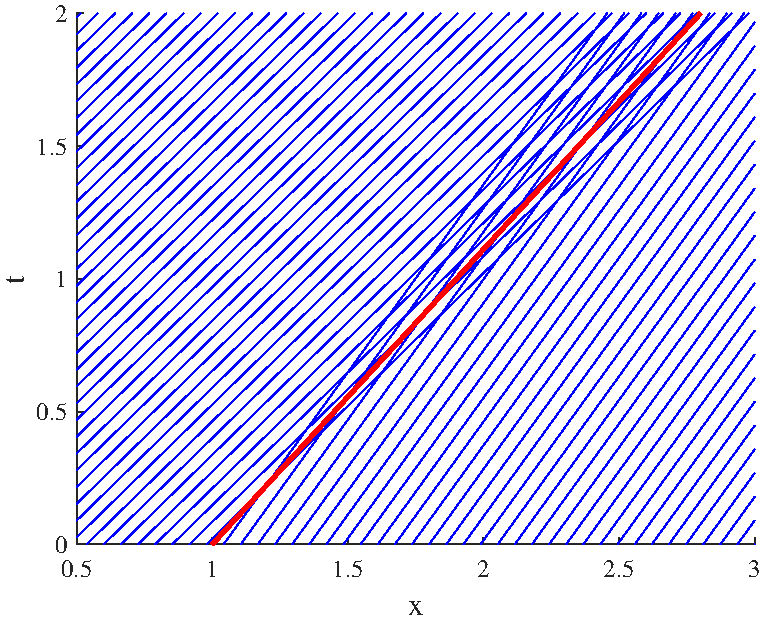
\includegraphics[width=\textwidth]{hw_14_plot1.pdf}
    \caption{Characteristics and $x_s$}
\end{figure}
\FloatBarrier
\subsection*{(d)}
The solution to the left of the shockline is a line at $u = \frac{\pi}{2}$, and to the right, a line at $u = \frac{\pi}{4}$. This is defined as: 
\begin{tcolorbox}[minipage,colback=white,arc=0pt,outer arc=0pt]
\begin{equation}
u(x,t) =
  \begin{cases}
			\frac{\pi}{2}, \; \; \; x < x_s \\
			\frac{\pi}{4} \; \; \; x \geq x_s \\
            \end{cases}
\
\end{equation}
\end{tcolorbox}
\subsection*{(e)}
If we change the characteristics in this way, the speed in the $u^+$ region is actually greater than it is in the $u^-$. As a result, the space between the solutions for $u$ actually increases in time, giving a growing region in which $u$ is not defined. 
\begin{figure}[!htbp]
  \centering
    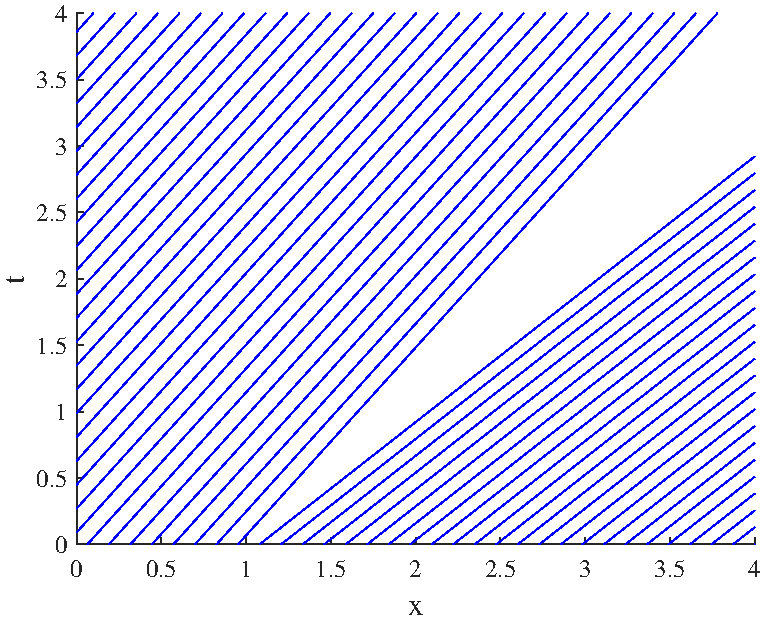
\includegraphics[width=\textwidth]{hw_14_plot2.pdf}
    \caption{$u^-=\frac{\pi}{4}$ and $u^+=\frac{\pi}{2}$}
\end{figure}
\FloatBarrier
\section*{Part 2}
\subsection*{(a)}
\begin{figure}[!htbp]
  \centering
    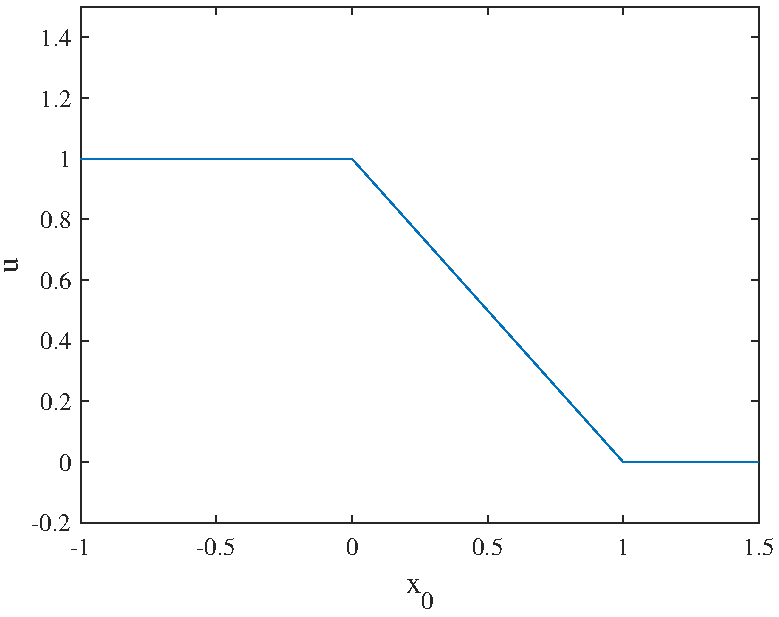
\includegraphics[width=\textwidth]{hw_14_plot3.pdf}
    \caption{$u(x, 0)$}
\end{figure}
\FloatBarrier
\subsection*{(b)}
First, we obtain the solution to $u$ along the characteristics:
\begin{equation}
\begin{aligned}
\frac{du}{dt} = 0\\
u(x(t), t) = A\\
A = u(x,0) = u_0(x_0)\\
\end{aligned}
\end{equation}
\begin{equation}
u(x(t),t) =
  \begin{cases}
			1, \; \; \; x_0 \leq 0 \\
			1-x_0, \; \; \; 0 < x_0 < 1\\
			0, \; \; \; x_0 \geq 1\\
            \end{cases}
\
\end{equation}
Using the values for $u_0(x_0)$ and $x(t) = x_0 + c(u_0(x_0))t$, we then obtain the characteristic curves:
\begin{tcolorbox}[minipage,colback=white,arc=0pt,outer arc=0pt]
\begin{equation}
x(t) =
  \begin{cases}
			x_0 + t, \; \; \; x_0 \leq 0 \\
			x_0 + t(1-x_0), \; \; \; 0 < x_0 < 1\\
			x_0, \; \; \; x_0 \geq 1\\
            \end{cases}
\
\end{equation}
\end{tcolorbox}
\subsection*{(c)}
We know from Knobel's and class that the breaking time is defined as the minimum of the equation:
\begin{equation}
t_b = \frac{-1}{c'(u_0(x_0))u'_0(x_0)}
\end{equation}
In this case, since $c(u_0(x_0)) = u_0(x_0)$ we know that $c'(u_0(x_0)) = 1$. This leaves $u'_0(x_0)$ which can easily be found from equations (15) and (16) above by taking the derivative in respect to $x_0$, which gives:
\begin{equation}
u'_0(x_0) =
  \begin{cases}
			0, \; \; \; x_0 \leq 0 \\
			-1, \; \; \; 0 < x_0 < 1\\
			0, \; \; \; x_0 \geq 1\\
            \end{cases}
\
\end{equation}
Plugging this into equation (18), it is clear that we can only minimize the equation using the middle region, which is constant, and results in $t_b = 1$, with an $x_0$ value that we can choose arbitrarily within the range of the minimized function. Because this middle region is defined from $0 < x_0 < 1$ we could choose an $x_0$ infinitely close to 0. We can then plug $t=1$ and $x_0 = 0$ into the correct domain of equation (17) to get $x = 0 + 1(1-0)$ (recall that this $x_0$ is actually defined in the $0 < x_0 <1$ region). Thus the breaking time occurs at:
\begin{tcolorbox}[minipage,colback=white,arc=0pt,outer arc=0pt]
\begin{equation}
t_b = 1, x = 1
\end{equation}
\end{tcolorbox}~
\\
\\
Alternatively, we can rigorously find the breaking time looking at the characteristics. The characteristics in the region $x \geq 1$ are just vertical lines at $x_0$, so the left-most one is a vertical line at $x = 1$. The characteristics in the domain $x_0 \leq 1$ have a slope of 1 and the right-most one is defined at $x_0 = 0$, thus it is a line with slope one that passes through the origin. This obviously crosses the $x_0 \geq 1$ line at $x = 1$. But what about the middle region?\\
\\
The middle region has a slope of $\frac{1}{1-x_0}$ and so because of the region of $x_0$ in which it's defined, we can see that the left-most line with the lowest slope, infinitely close to $x_0 = 0$, will not cross the last characteristic in the left region (it will basically be the same line going to the same $x_0$). The rightmost one does not cross the line at $x_0=0$ for the same reason, but oviously cross the last characteristic from the left region at $x=0$. But what about the middle region characteristics crossing each other, or the rest of the characteristics crossing with the right or left region?\\
\\
The middle region in terms of x is defined by $t = \frac{x - x_0}{1-x_0}$. Suppose we arbitrarily pick any two lines (or any three, or even an infinite number) of lines in this region, defined by two different $x_0$ values, say $x_1$ and $x_2$. Let's assume they cross, since geometrically, it would appear they all cross at the same place:
\begin{equation}
\frac{x-x_2}{1-x_2} = \frac{x-x_1}{1-x_1}
\end{equation}
Since this is sort of an aside, I won't show all the algebra, but it's pretty simple and quickly reduces to x = 1. This means that all the lines in this middle region cross at at this x value. Furthermore, they all cross at this x value at $t=1$, since we then have $t = \frac{1 - x_0}{1 - x_0}$. And since they are lines, none of them crosses $x_0 = 1$ before this point, meaning none of them crosses the characteristics of the right region, or the last characteristic of the left region, until they all cross each other at $x = 1, t = 1$. Sorry if this geometric version is redundant, but I got to thinking about it and figured I'd include it.
\subsection*{(d)}
Using equation (16) above, we can solve for $x_0$ for each of the 3 ranges. $x_0 \leq 0$ and $x_0 \geq 0$ are fairly straightforward, so I won't show my work for those. For $0 < x_0 < 1$ however, we have the following:
\begin{equation}
\begin{aligned}
x(t) = x_0 + t(1-x_0)\\
\frac{x}{x_0} = 1 - t + \frac{t}{x_0}\\
\frac{x}{x_0} - \frac{t}{x_0} = 1 - t\\
\frac{1}{x_0}(x - t) = 1 -t\\
x_0 = \frac{x -t}{1-t}
\end{aligned}
\end{equation}
We then have:
\begin{equation}
x_0 =
  \begin{cases}
			x - t, \; \; \; x_0 \leq 0 \\
			\frac{x -t}{1-t}, \; \; \; 0 < x_0 < 1\\
			x, \; \; \; x_0 \geq 1\\
            \end{cases}
\
\end{equation}
We can then substitute these values into equation (16) to obtain the solution for $t < t_b$. Again, the substitutions are fairly straightforward, but I will show the work for $0 < x_0 < 1$.
\begin{equation}
\begin{aligned}
0 < \frac{x -t}{1-t} < 1\\
0 < x - t < 1 - t\\
t < x < 1
\end{aligned}
\end{equation}
And finally substituting all this into (15) gives the solution for $0 \leq t < t_b$. We can see in this solution that the middle constraint solutions only exist in a range between $t=0$, $x = 1$ and $t = x$, as described in part (c).
\begin{tcolorbox}[minipage,colback=white,arc=0pt,outer arc=0pt]
\begin{equation}
u(x,t) = 
  \begin{cases}
			1, \; \; \; x \leq t \\
			1-\frac{x -t}{1-t}, \; \; \; t < x < 1\\
			0, \; \; \; x \geq 1\\
            \end{cases}
\
\end{equation}
\end{tcolorbox}
\subsection*{(e)}
We can see from the stated problem that $\phi_x = uu_x$. Integrating this gives
\begin{equation}
\phi = \frac{u^2}{2}
\end{equation}
Considering equation (22) above, we can see that at the breaking time $t_b = 1$, the solution is defined in two regions as the second constraint $t < x < 1$ is not satisfied for any $t > t_b = 1$. This leaves the other two constraints:
\begin{equation}
\begin{aligned}
u^- = 1, \; x < t\\
u^+ = 0, \; x > 1
\end{aligned}
\end{equation}
With this information we can then use the Rankine-Hugoniot relation:
\begin{equation}
\begin{aligned}
\frac{dx_0}{dt} = \frac{\frac{0^2}{2} - \frac{1^2}{2}}{0 - 1}\\
\frac{dx_0}{dt} = \frac{1}{2}\\
x_s(t) = \frac{1}{2}t + C\\
x_s(1) = 1  = \frac{1}{2}(1) + C\\
\end{aligned}
\end{equation}
\begin{tcolorbox}[minipage,colback=white,arc=0pt,outer arc=0pt]
\begin{equation}
x_s(t) = \frac{1}{2}t + \frac{1}{2}
\end{equation}
\end{tcolorbox}
\subsection*{(f)}
Making use equations (22), (24), and (25) above:
\begin{equation}
  u(x,t)=
  \begin{cases}
    \begin{cases}
      1, & x \leq t \\
      1 - \frac{x-t}{1-t}, & t < x < 1\\
      0, & x \geq 1
    \end{cases}
    &0 < t < 1\\
    \begin{cases}
      1,  & x < x_s(t) \\
      0,  & x > x_s(t)
    \end{cases}
    &t\geq 1
  \end{cases}
\end{equation}
\textbf{(g)}
\begin{figure}[H]
  \centering
  \begin{minipage}[b]{0.49\textwidth}
    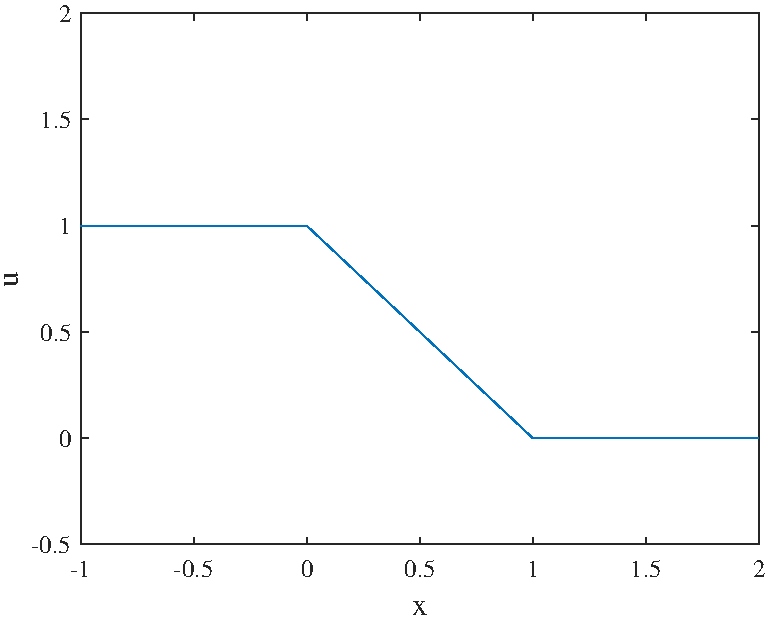
\includegraphics[width=\textwidth]{hw_14_plot5.pdf}
    \caption{$t = 0$}

  \end{minipage}
  \hfill
  \begin{minipage}[b]{0.49\textwidth}
    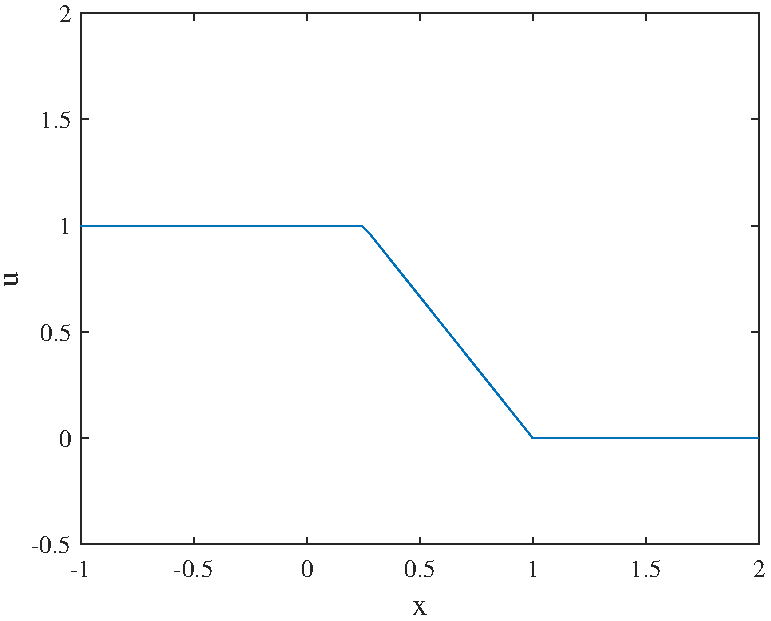
\includegraphics[width=\textwidth]{hw_14_plot6.pdf}
    \caption{$t = 0.25$}

  \end{minipage}
    \hfill
  \begin{minipage}[b]{0.49\textwidth}
    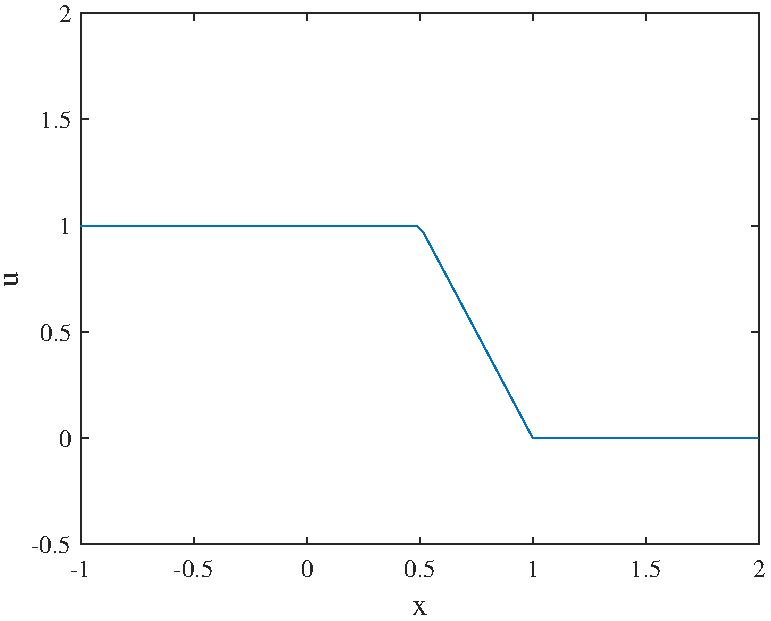
\includegraphics[width=\textwidth]{hw_14_plot7.pdf}
    \caption{$t = 0.5$}

  \end{minipage}
    \hfill
  \begin{minipage}[b]{0.49\textwidth}
    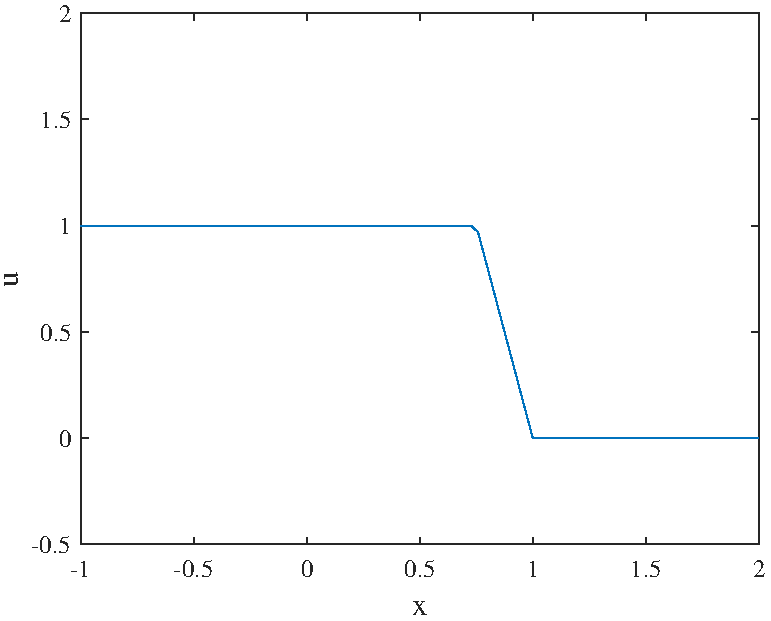
\includegraphics[width=\textwidth]{hw_14_plot8.pdf}
    \caption{$t = .75$}

  \end{minipage}
      \hfill
  \begin{minipage}[b]{0.49\textwidth}
    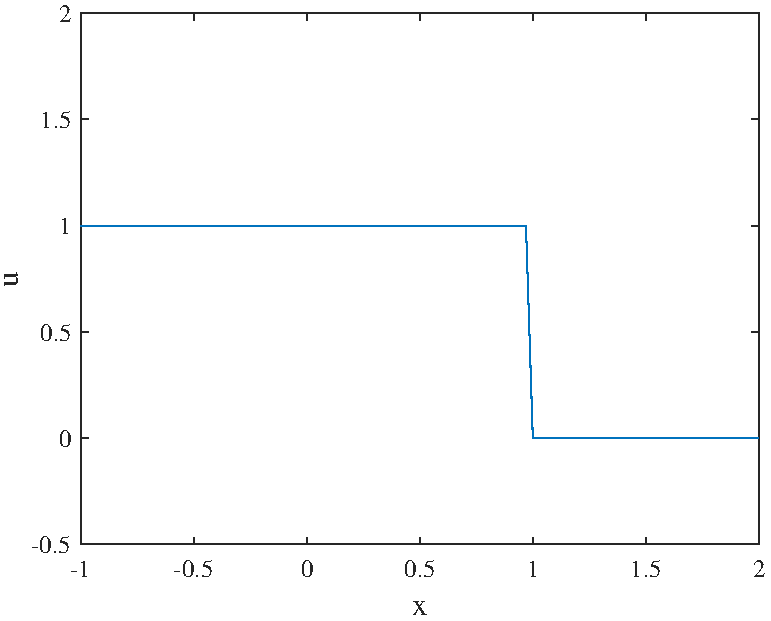
\includegraphics[width=\textwidth]{hw_14_plot9.pdf}
    \caption{$t = 1$}

  \end{minipage}
      \hfill
  \begin{minipage}[b]{0.49\textwidth}
    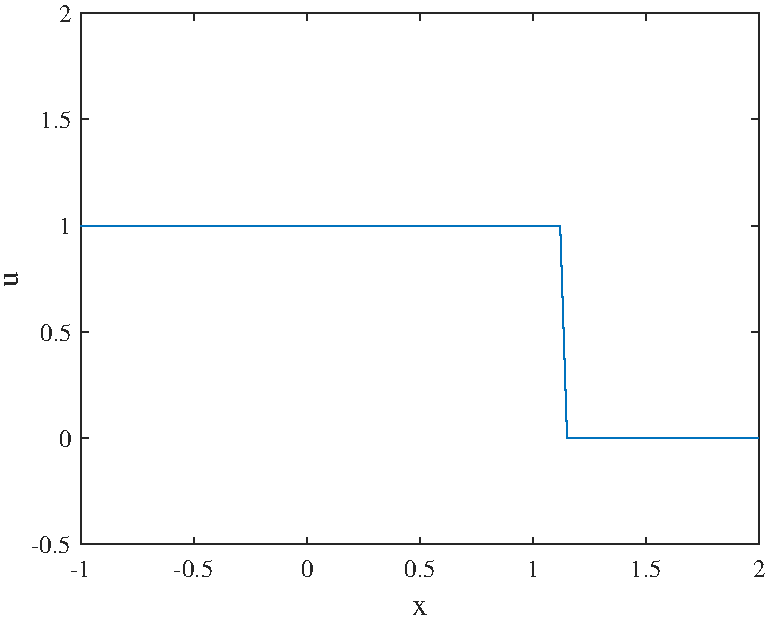
\includegraphics[width=\textwidth]{hw_14_plot10.pdf}
    \caption{$t = 1.25$}

  \end{minipage}
    \hfill
  \begin{minipage}[b]{0.49\textwidth}
    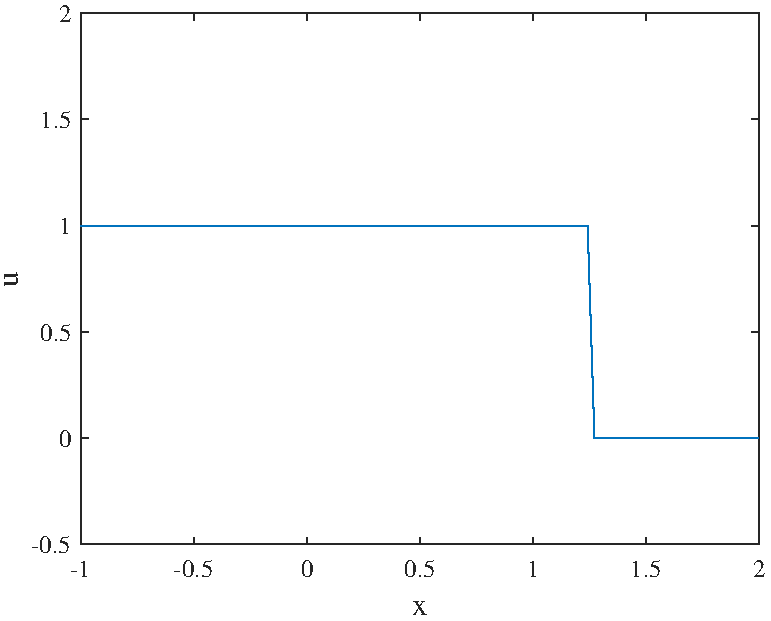
\includegraphics[width=\textwidth]{hw_14_plot11.pdf}
    \caption{$t = 1.5$}

  \end{minipage}
      \hfill
  \begin{minipage}[b]{0.49\textwidth}
    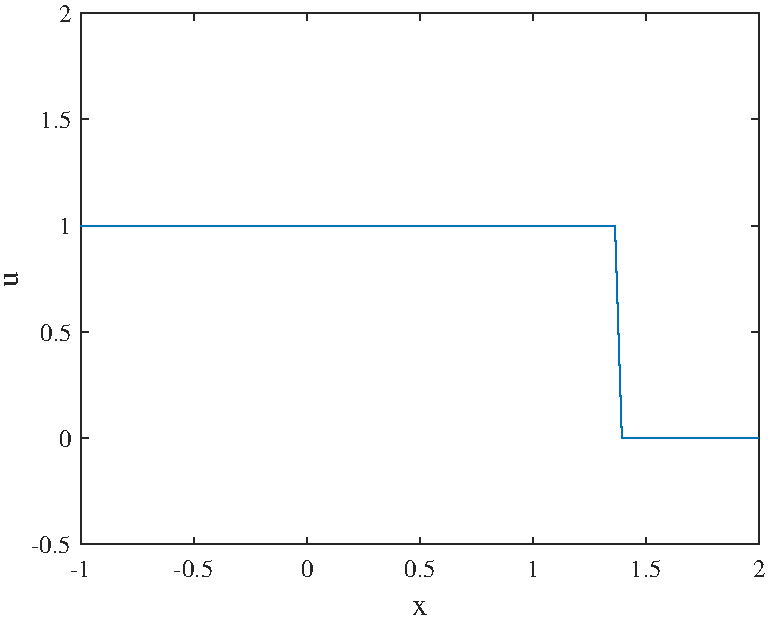
\includegraphics[width=\textwidth]{hw_14_plot12.pdf}
    \caption{$t = 1.75$}

  \end{minipage}
\end{figure}
\begin{figure}[!htbp]
  \centering
    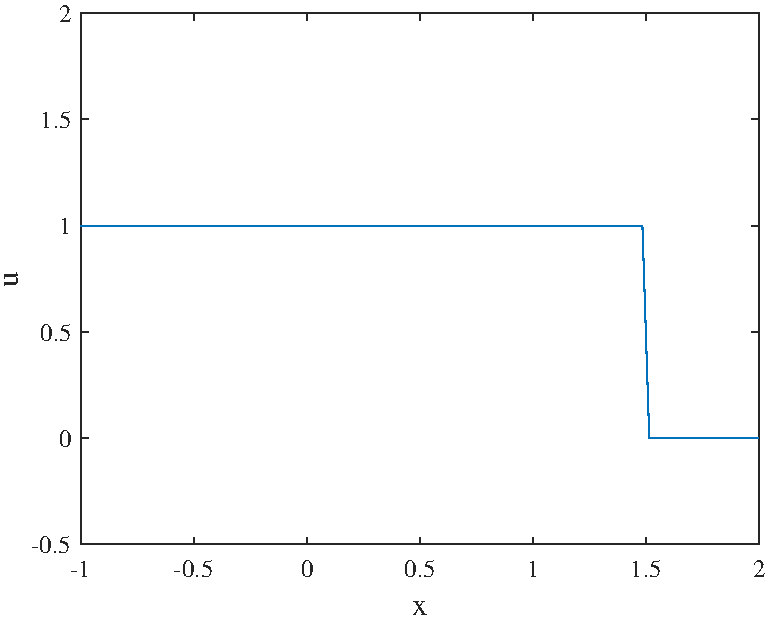
\includegraphics[width=.49\textwidth]{hw_14_plot13.pdf}
    \caption{$t = 2$}
\end{figure}
\section*{Part 3}
\subsection*{(a)}
For these values, there is no change in density of cars at any point, thus no shock/traffic jam forms. Traffic travels forward at a uniform speed of $v = v_1(1 - \frac{\frac{u_1}{3}}{u_1}) = \frac{2}{3}v_1$. This is the best scenario for the flow of traffic. 
\begin{figure}[!htbp]
  \centering
    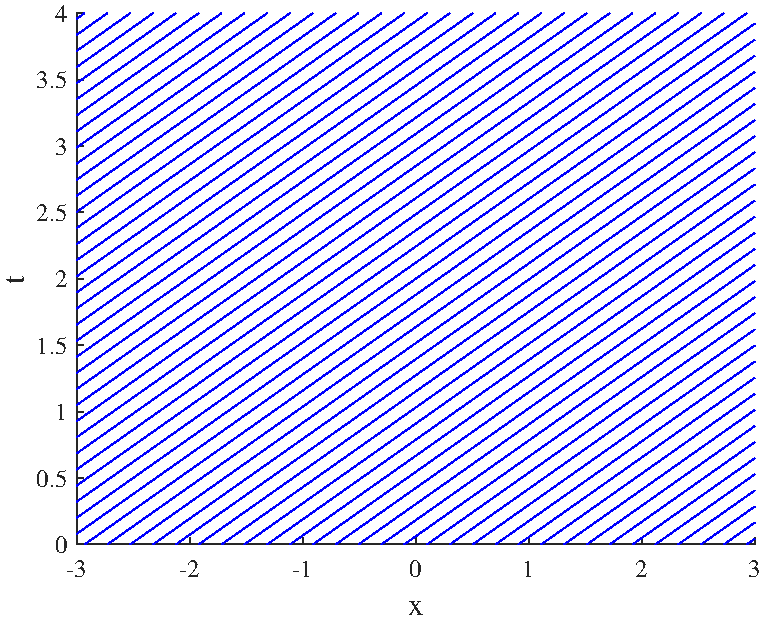
\includegraphics[width=.49\textwidth]{hw_14_plot14.pdf}
    \caption{}
\end{figure}
\subsection*{(b)}

For these values a traffic jam forms immediately at $t=0$. If you zoom in on the graph, it seems like the information (i.e. the traffic jam) is traveling forward, which makes sense since the $u^+$ value is less than $u_1$. Overall this means traffic hits the traffic jam and then immediately slows to a much lower speed. This is not a good scenario for traffic flow. Information is moving forward i.e. traffic is moving slowly forward, at the following rate:
\begin{equation}
\begin{aligned}
\phi = v_1(u - \frac{u^2}{u_1})\\
\phi^+ = v_1(\frac{2u_1}{3} - \frac{(\frac{2u_1}{3})^2}{u_1}\\
\phi^+ = v_1(\frac{2u_1}{3} - \frac{4u_1}{9}) = \frac{2}{9}v_1u_1\\
\phi^- = v_1(\frac{u_1}{6} - \frac{(\frac{u_1}{6})^2}{u_1}\\
\phi^- = v_1(\frac{u_1}{6} - \frac{u_1}{36}) = \frac{5}{36}v_1u_1\\
\end{aligned}
\end{equation}
Then using this to calculate the slope of the shock line we have:
\begin{equation}
\begin{aligned}
\frac{dx_s}{dt} = \frac{\frac{2u_1v_1}{9} - \frac{5u_1v_1}{36}}{\frac{2u_1}{3} - \frac{u1}{6}}\\
\frac{dx_s}{dt} = 2\frac{1}{u_1}( \frac{2u_1v_1}{9} - \frac{5u_1v_1}{36})\\
\frac{dx_s}{dt} = \frac{4}{9}v_1 - \frac{10}{36}v_1\\
\end{aligned}
\end{equation}
\begin{tcolorbox}[minipage,colback=white,arc=0pt,outer arc=0pt]
\begin{equation}
\frac{dx_s}{dt} = \frac{v_1}{6}
\end{equation}
\end{tcolorbox}
\begin{figure}[!htbp]
  \centering
    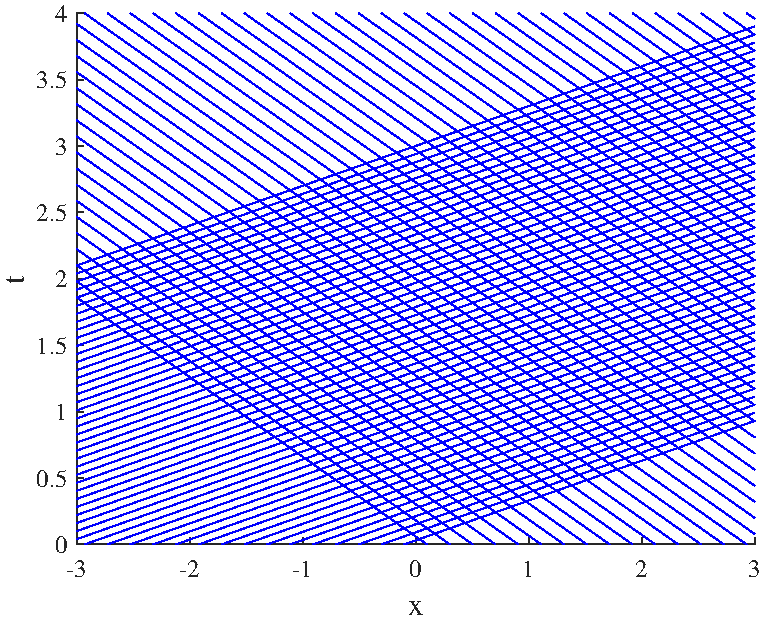
\includegraphics[width=.49\textwidth]{hw_14_plot15.pdf}
    \caption{}
\end{figure}
\FloatBarrier

\subsection*{(c)}
For these values, traffic is moving more slowly on the left and more quickly on the right, and thus a region forms in which there are no characteristics, and thus no solution to $u$. Intuitively, this would seem to model an area in which there are no cars, but not in any useful way since the area is growing moving \textit{backwards} as well as forwards. As to why this would happen, I'm not sure. I suppose it could model an expanding work crew diverting traffic to a side street.
\begin{figure}[!htbp]
  \centering
    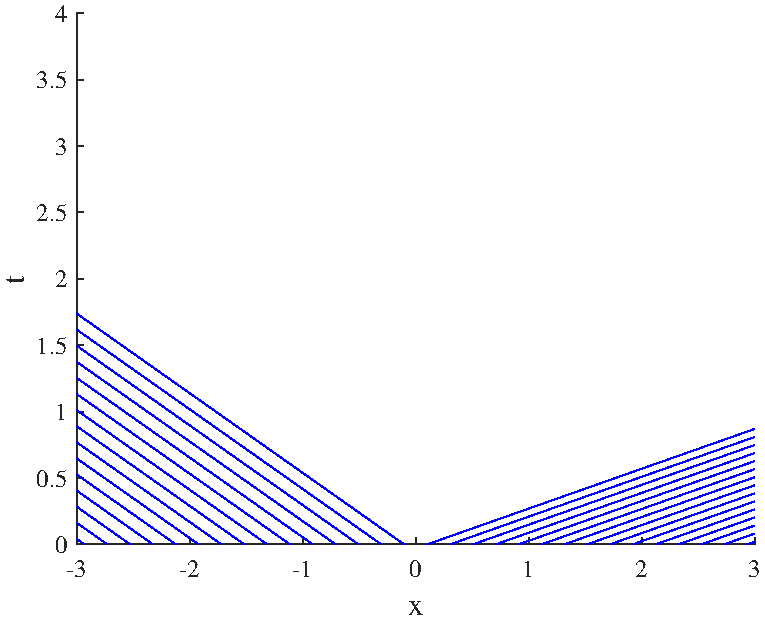
\includegraphics[width=.49\textwidth]{hw_14_plot16.pdf}
    \caption{}
\end{figure}
\FloatBarrier
\subsection*{(d)}
% also need to observe that both slopes need to have the same sign in order for shocks to form.

The slope of the characteristics in the traffic problem are give by 
\begin{equation}
\frac{1}{v_1(1-\frac{2u^{\pm}}{u_1})}
\end{equation}
We can see that when the slope of the characteristics in the left region are greater than the ones in the right, they will cross (regardless of whether the slopes are positive or negative). We then have:
\begin{equation}
\frac{1}{v_1(1-\frac{2u^-}{u_1})} > \frac{1}{v_1(1-\frac{2u^+}{u_1})}
\end{equation}
This then very quickly simplifies down to $u^+ \geq u^-$, which is to say if the initial density is higher in the right region than it is on the left region, a shock will form. This also correctly deals with the scenario in which the density on the left is higher than the right, in which the characteristics are going away from each other. In that situation, the characteristics in the left region have lower slope than those in the right, up to and including opposite sign. While implied above, we should note explicitly that when the slopes are equal, no shock will form. 
\end{document}
